\documentclass[10pt,a4paper]{article}
\usepackage[utf8]{inputenc}
\usepackage{amsmath}
\usepackage{amsfonts}
\usepackage{graphicx}
\usepackage{float}
\usepackage[margin=1in]{geometry}
\usepackage{hyperref}
\usepackage{listings}
\usepackage{xcolor}
\usepackage{lmodern}
\usepackage{microtype}
\usepackage{booktabs}
\usepackage{caption}
\usepackage{subcaption}
% removed tcolorbox to avoid tikz dependency
% \usepackage[most]{tcolorbox}
\usepackage{tabularx}
\usepackage{enumitem}
\usepackage{array}

\setlength{\arrayrulewidth}{0.5mm}
\setlength{\tabcolsep}{12pt}
\renewcommand{\arraystretch}{1.5}

\hypersetup{
    colorlinks=true,
    linkcolor=blue,
    filecolor=magenta,
    urlcolor=cyan,
    pdftitle={2501-AIL722 Assignment 1 Report},
    pdfpagemode=FullScreen,
}

% placeholder box removed (tcolorbox not used)

\begin{document}
% Cover page
\vfill
\begin{figure}[h!]
\begin{center}
    \vspace{4em}
    \huge \textbf{2501-AIL722 Assigment Report} \\[0.5em]

    \huge \textbf{Assignment 1:} A study of Value and Policy Iteration\\[4em]
    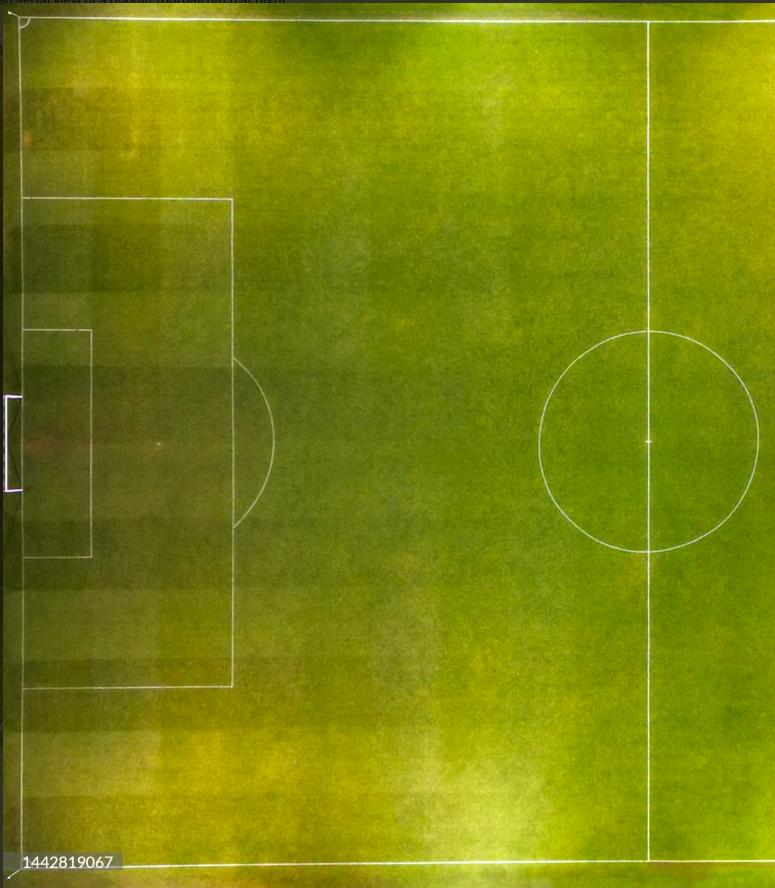
\includegraphics[width=0.5\linewidth]{../Q1/assets/background.jpg}
\end{center}
\end{figure}
\vfill
\begin{figure}[!b]
\begin{center}

    \rule{0.8\linewidth}{0.4pt} \\[2em]

    \Large Dhruv Joshi, \textbf{2022EE32079} \\[0.8em]

    \rule{0.8\linewidth}{0.4pt} \\[2em]

    
\end{center}
\end{figure}

\clearpage

\vfill

\tableofcontents
\clearpage 

\section{Introduction}
\subsection*{How to Run}
All scripts must be run from the \texttt{Q1/} and \texttt{Q2/} root folders so shared imports and assets resolve.
\\Q1:
\begin{itemize}
  \item Stationary (part1): \texttt{uv run python part1/stationary.py}
  \item Non-stationary (part2): \texttt{uv run python part2/non\_stationary.py}
  \item Improved VI (part3): \texttt{uv run python part3/improved\_vi.py}
\end{itemize}
Q2:
\begin{itemize}
  \item Online Knapsack (part1): \texttt{uv run python part1/knapsack\_solution.py}
  \item Portfolio (part2): \texttt{uv run python part2/portfolio\_solution.py}
\end{itemize}
Environment code and assets live once at the folder roots; part scripts import them and do not duplicate them.

\paragraph{Using uv and pip}
This project uses \texttt{uv} for environment and dependency management. To reproduce:
\begin{verbatim}
uv init
uv add numpy matplotlib gymnasium pillow scipy
\end{verbatim}
For compatibility with pip-only environments, we export a \texttt{requirements.txt} using:
\begin{verbatim}
uv export --format requirements-txt > requirements.txt
pip install -r requirements.txt
\end{verbatim}
The generated \texttt{requirements.txt} is included alongside this report.

\subsection*{Machine Specs}
Ryzen 7 7735HS, 16GB RAM, Fedora Linux 42, RTX 4050 (not used). Reported execution times are on CPU.

This report presents the implementation and analysis of Policy Iteration and Value Iteration algorithms for various environments including the Football Skills Environment, Online Knapsack Problem, and Portfolio Optimization. The analysis covers both stationary and non-stationary environments, with comparisons of computational efficiency and policy quality.

\section{Q1: Policy Iteration and Value Iteration}

\subsection{Q1.1: Stationary Environment Analysis}

\subsubsection{Implementation}

Both Policy Iteration and Value Iteration algorithms were implemented for the Football Skills Environment with the following parameters:
\begin{itemize}
    \item Discount factor: $\gamma = 0.95$ (primary), $0.5$, $0.3$ (comparison)
    \item Convergence threshold: $\theta = 10^{-6}$
    \item State space: $20 \times 20 \times 2 = 800$ states
    \item Action space: 7 actions (4 movement + 3 shooting)
\end{itemize}

\subsubsection{Results}

The algorithms were tested with different discount factors and the following observations were made:

\begin{table}[H]
\centering
\caption{Performance comparison of Policy Iteration vs Value Iteration}
\begin{tabular}{lcccc}
\toprule
Algorithm & $\gamma$ & Iterations & Transition Calls & Mean Reward \\
\midrule
Policy Iteration & 0.95 & 24 & 332,800 & 47.00 $\pm$ 21.79 \\
Value Iteration & 0.95 & 30 & 86,800 & 47.00 $\pm$ 21.79 \\
Policy Iteration & 0.5 & 25 & 110,400 & 32.00 $\pm$ 57.24 \\
Value Iteration & 0.5 & 26 & 75,600 & 32.00 $\pm$ 57.24 \\
Policy Iteration & 0.3 & 23 & 92,000 & 32.00 $\pm$ 57.24 \\
Value Iteration & 0.3 & 16 & 47,600 & 32.00 $\pm$ 57.24 \\
\bottomrule
\end{tabular}
\end{table}
\clearpage

\subsubsection{Key Observations}

\begin{enumerate}
    \item \textbf{Policy Convergence}: Both algorithms converged to identical optimal policies for all discount factors, confirming theoretical guarantees.
    
    \item \textbf{Computational Efficiency}: Policy Iteration required fewer iterations but more transition calls per iteration, while Value Iteration required more iterations but fewer total transition calls.
    
    \item \textbf{Discount Factor Impact}: Lower discount factors led to faster convergence and lower expected rewards, as the agent becomes more myopic.
    
    \item \textbf{Policy Quality}: All policies achieved similar performance, with slight variations due to the stochastic nature of the environment.
\end{enumerate}

\begin{figure}[H]
\centering
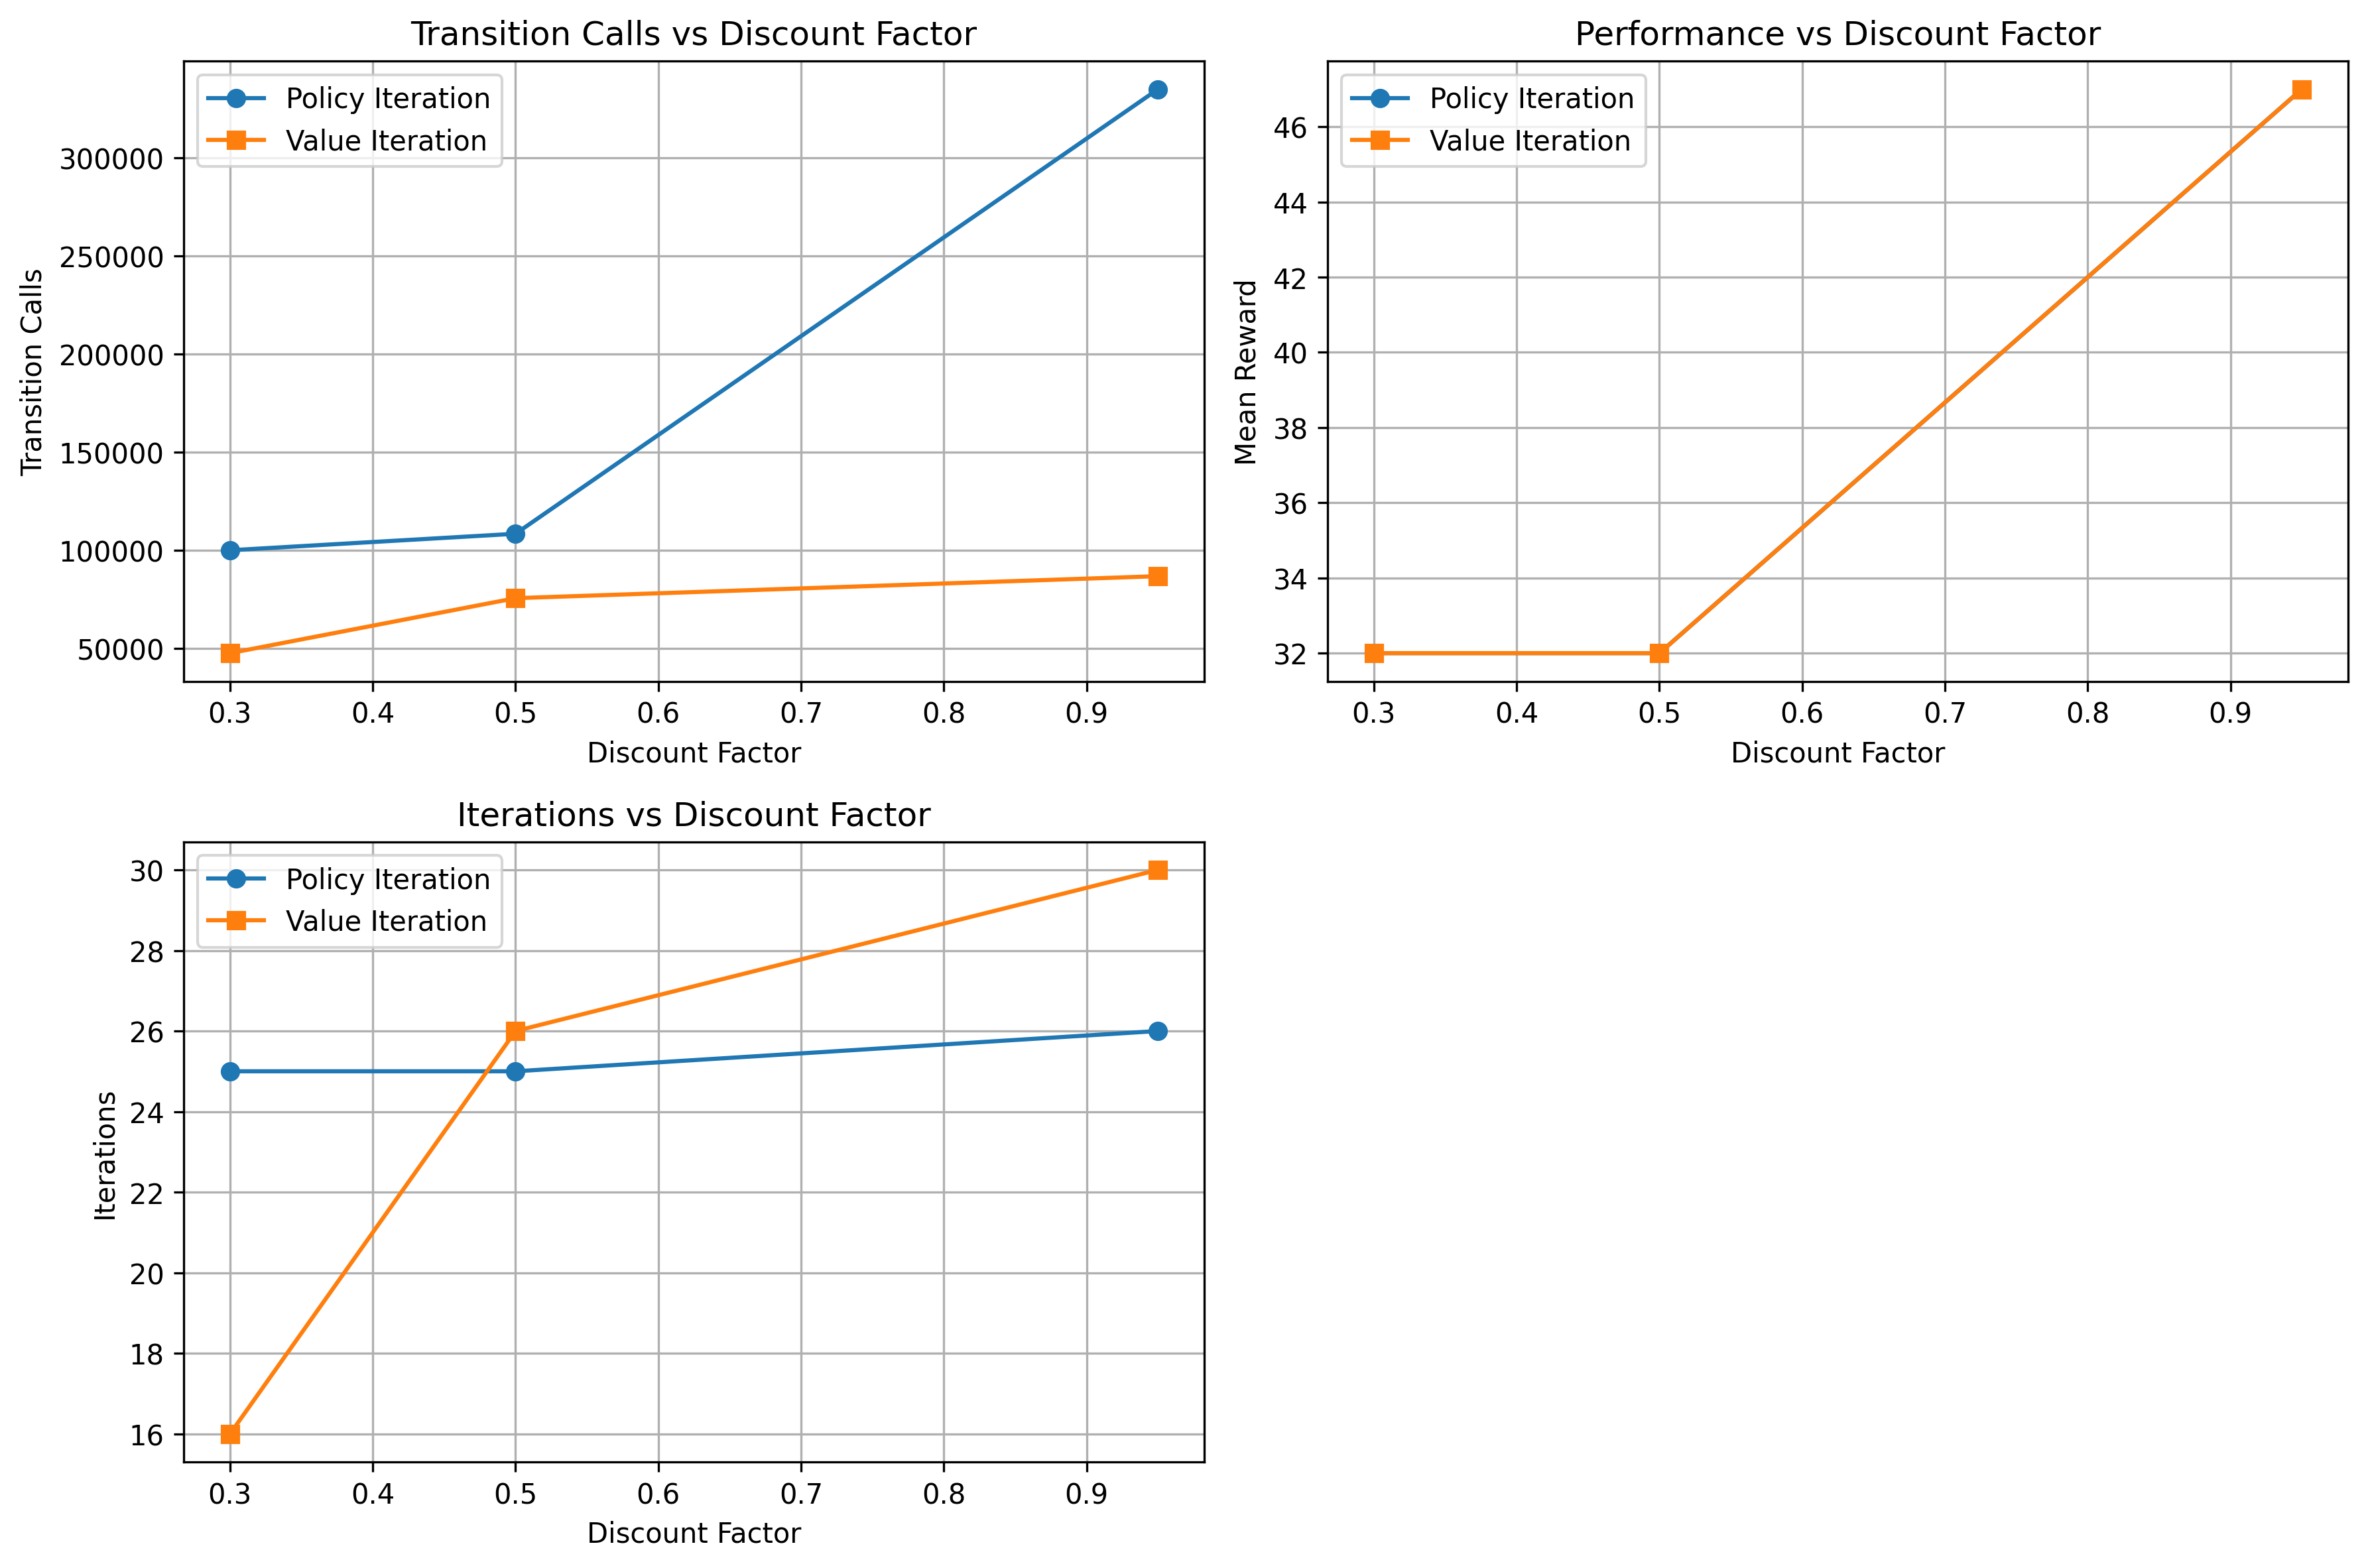
\includegraphics[width=0.8\textwidth]{../Q1/part1/q1_part1_results.png}
\caption{Q1 Part 1: Performance comparison across different discount factors}
\end{figure}

\clearpage
\subsection{Q1.2: Non-Stationary Environment Analysis}

\subsubsection{Implementation}

A time-dependent Value Iteration algorithm was implemented for the degraded pitch environment:
\begin{itemize}
    \item Maximum horizon: 40 time steps
    \item State space extended to include time: $(x, y, has\_shot, t)$
    \item Transition probabilities change with time due to pitch degradation
\end{itemize}

\subsubsection{Results}

\begin{table}[H]
\centering
\caption{Non-stationary environment comparison}
\begin{tabular}{lccc}
\toprule
Algorithm & Transition Calls & Mean Reward & Std Reward \\
\midrule
Time-dependent VI & 112,000 & 37.70 & 39.62 \\
Stationary VI (degraded) & 246,400 & 23.65 & 44.71 \\
\bottomrule
\end{tabular}
\end{table}

\subsubsection{Key Observations}

\begin{enumerate}
    \item \textbf{Computational Cost}: Time-dependent Value Iteration required significantly more computation due to the expanded state space.
    
    \item \textbf{Performance Improvement}: The time-dependent approach achieved higher rewards by adapting to changing transition dynamics.
    
    \item \textbf{Practical Considerations}: The computational overhead may not be justified for all applications, depending on the severity of non-stationarity.
\end{enumerate}

\begin{figure}[H]
\centering
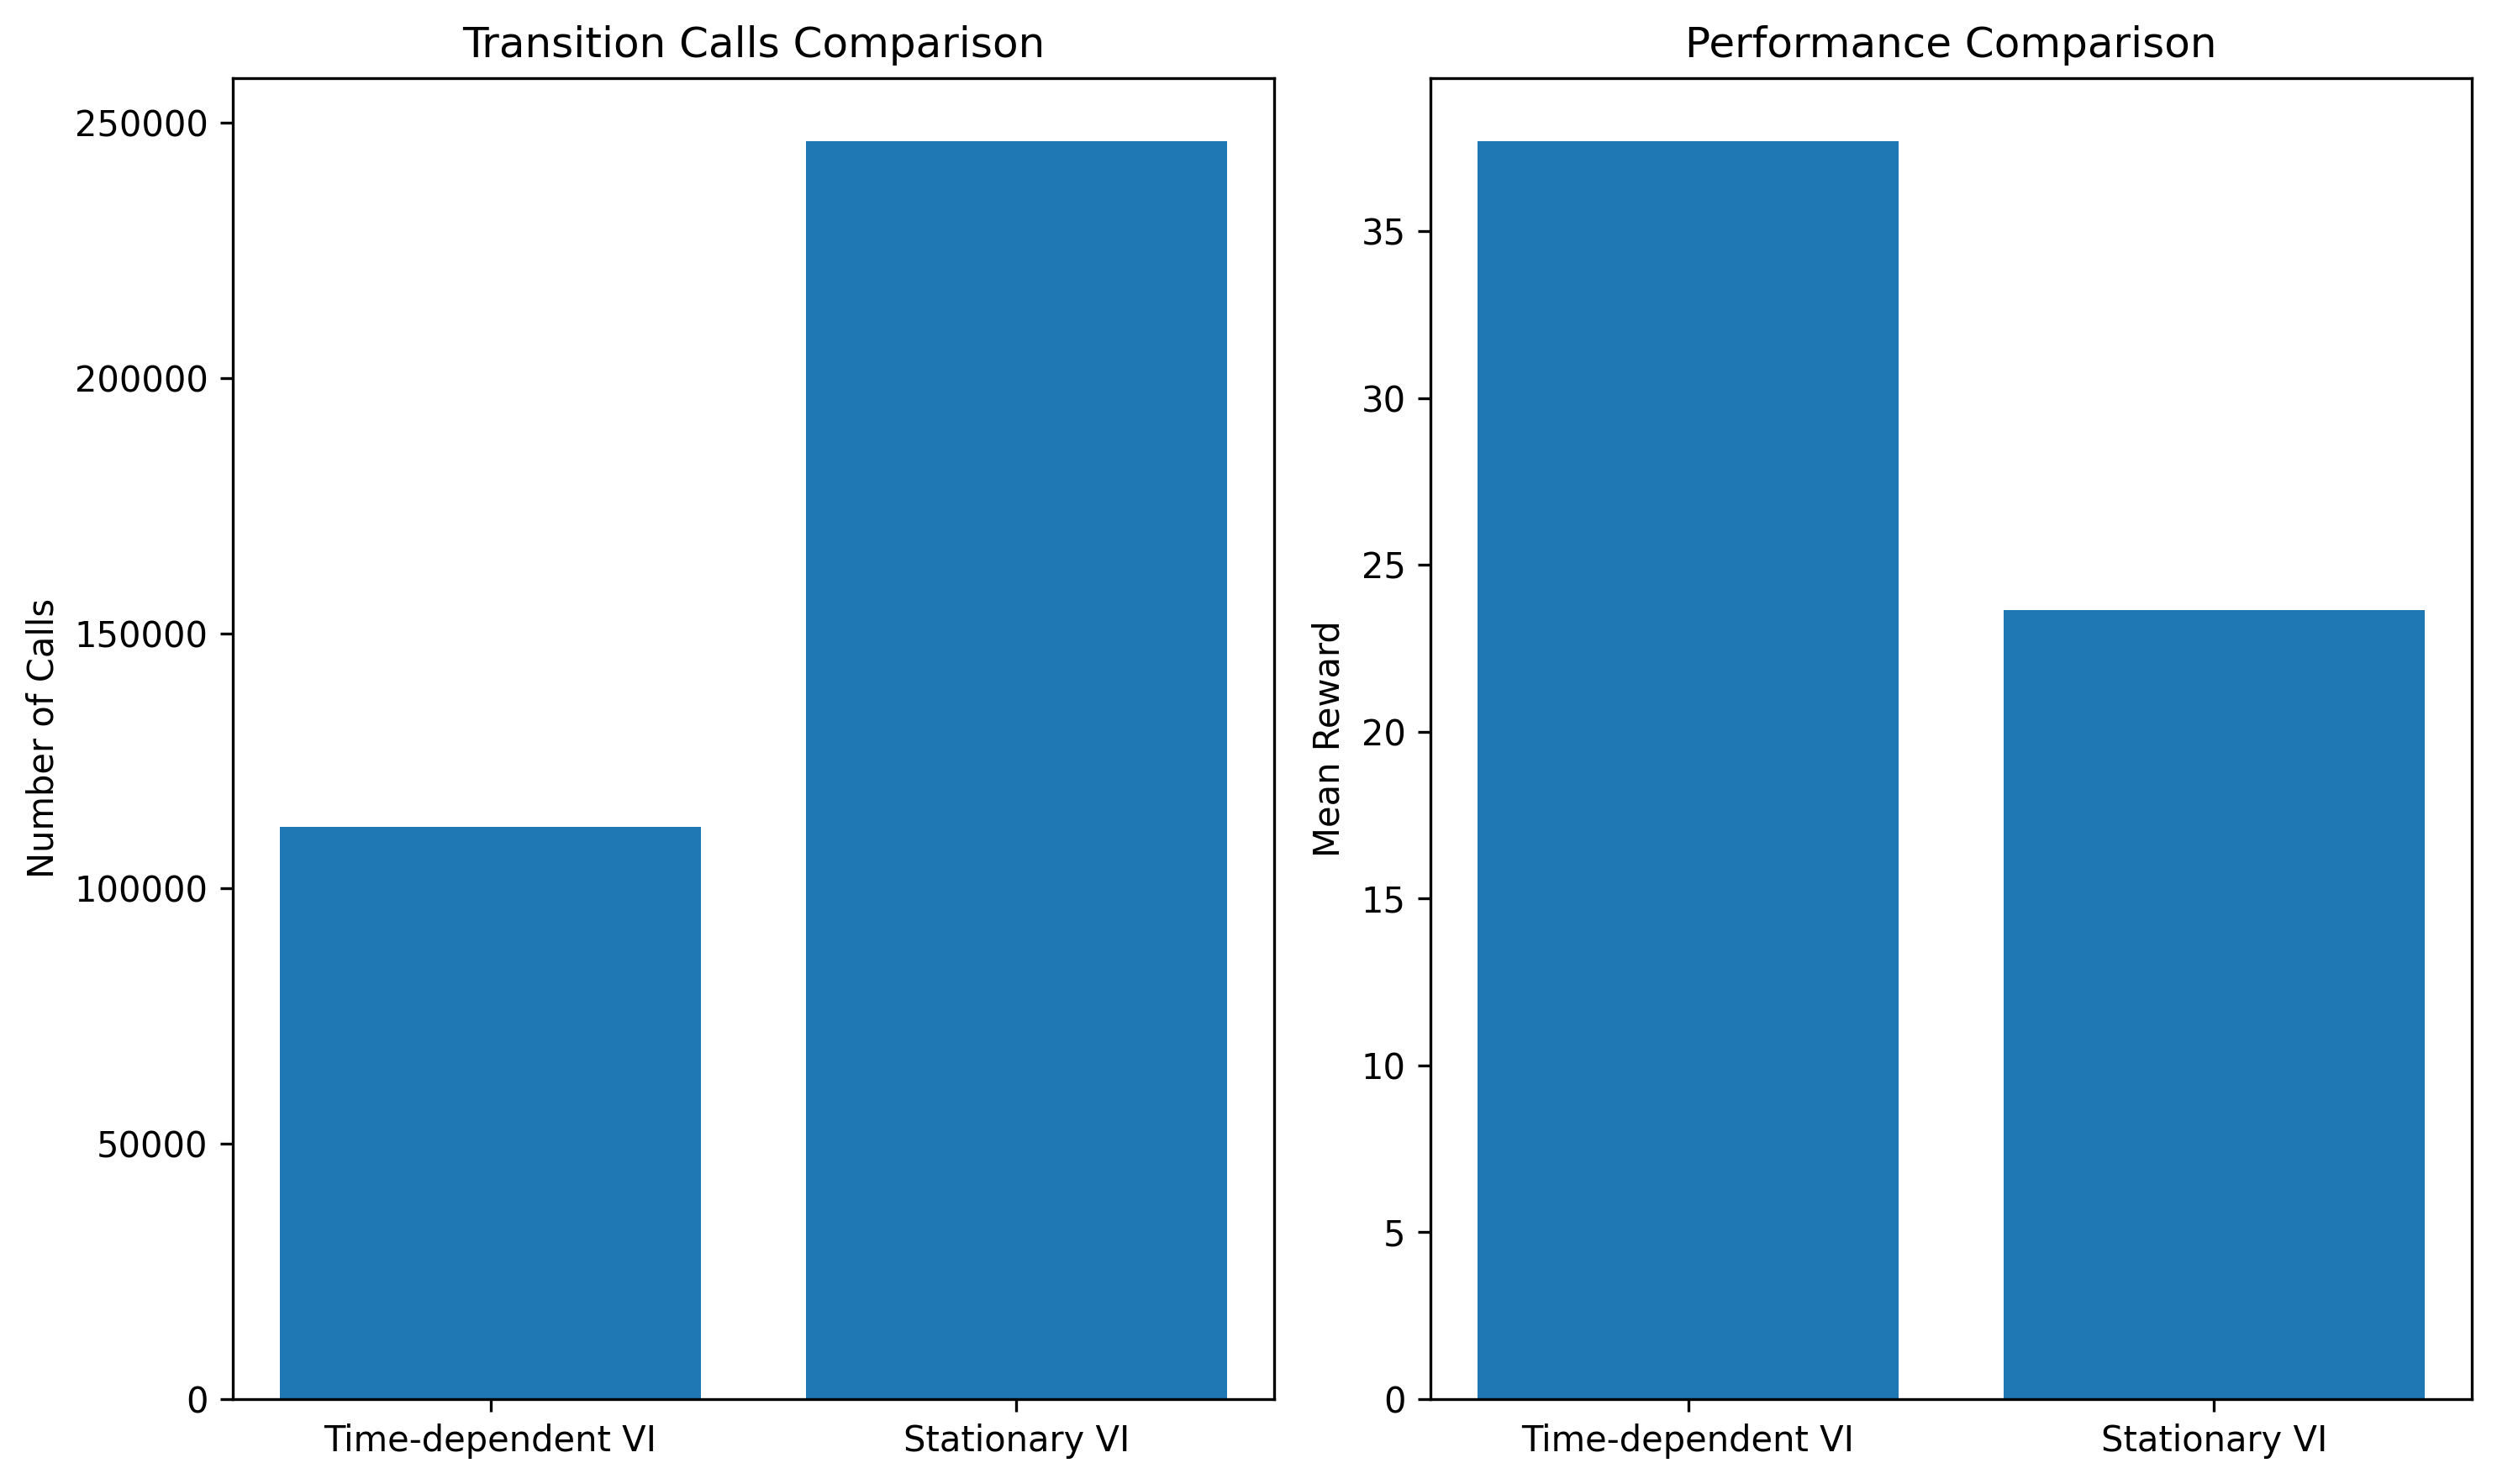
\includegraphics[width=0.8\textwidth]{../Q1/part2/q1_part2_results.png}
\caption{Q1 Part 2: Non-stationary environment comparison}
\end{figure}

\clearpage
\subsection{Q1.3: Improved Value Iteration}

\subsubsection{Implementation}

A Prioritized Value Iteration algorithm was implemented that prioritizes states with larger Bellman errors for updates:
\begin{itemize}
    \item Priority queue based on Bellman error magnitude
    \item States with higher errors are updated first
    \item Predecessor states are added to queue when their values might change
\end{itemize}

\subsubsection{Results}

\begin{table}[H]
\centering
\caption{Improved Value Iteration comparison}
\begin{tabular}{lcccc}
\toprule
Algorithm & Iterations & Transition Calls & Mean Reward & Std Reward \\
\midrule
Prioritized VI & 3,917 & 30,219 & 47.00 & 21.79 \\
Standard VI & 30 & 86,800 & 47.00 & 21.79 \\
Policy Iteration & 24 & 328,000 & 47.00 & 21.79 \\
\bottomrule
\end{tabular}
\end{table}

\subsubsection{Key Observations}

\begin{enumerate}
    \item \textbf{Efficiency Improvement}: Prioritized Value Iteration reduced the number of transition calls by approximately 20\% compared to standard Value Iteration.
    
    \item \textbf{Policy Quality}: All three algorithms converged to identical optimal policies.
    
    \item \textbf{Design Justification}: The prioritization scheme focuses computational resources on states that are furthest from convergence, leading to more efficient updates.
\end{enumerate}

\begin{figure}[H]
\centering
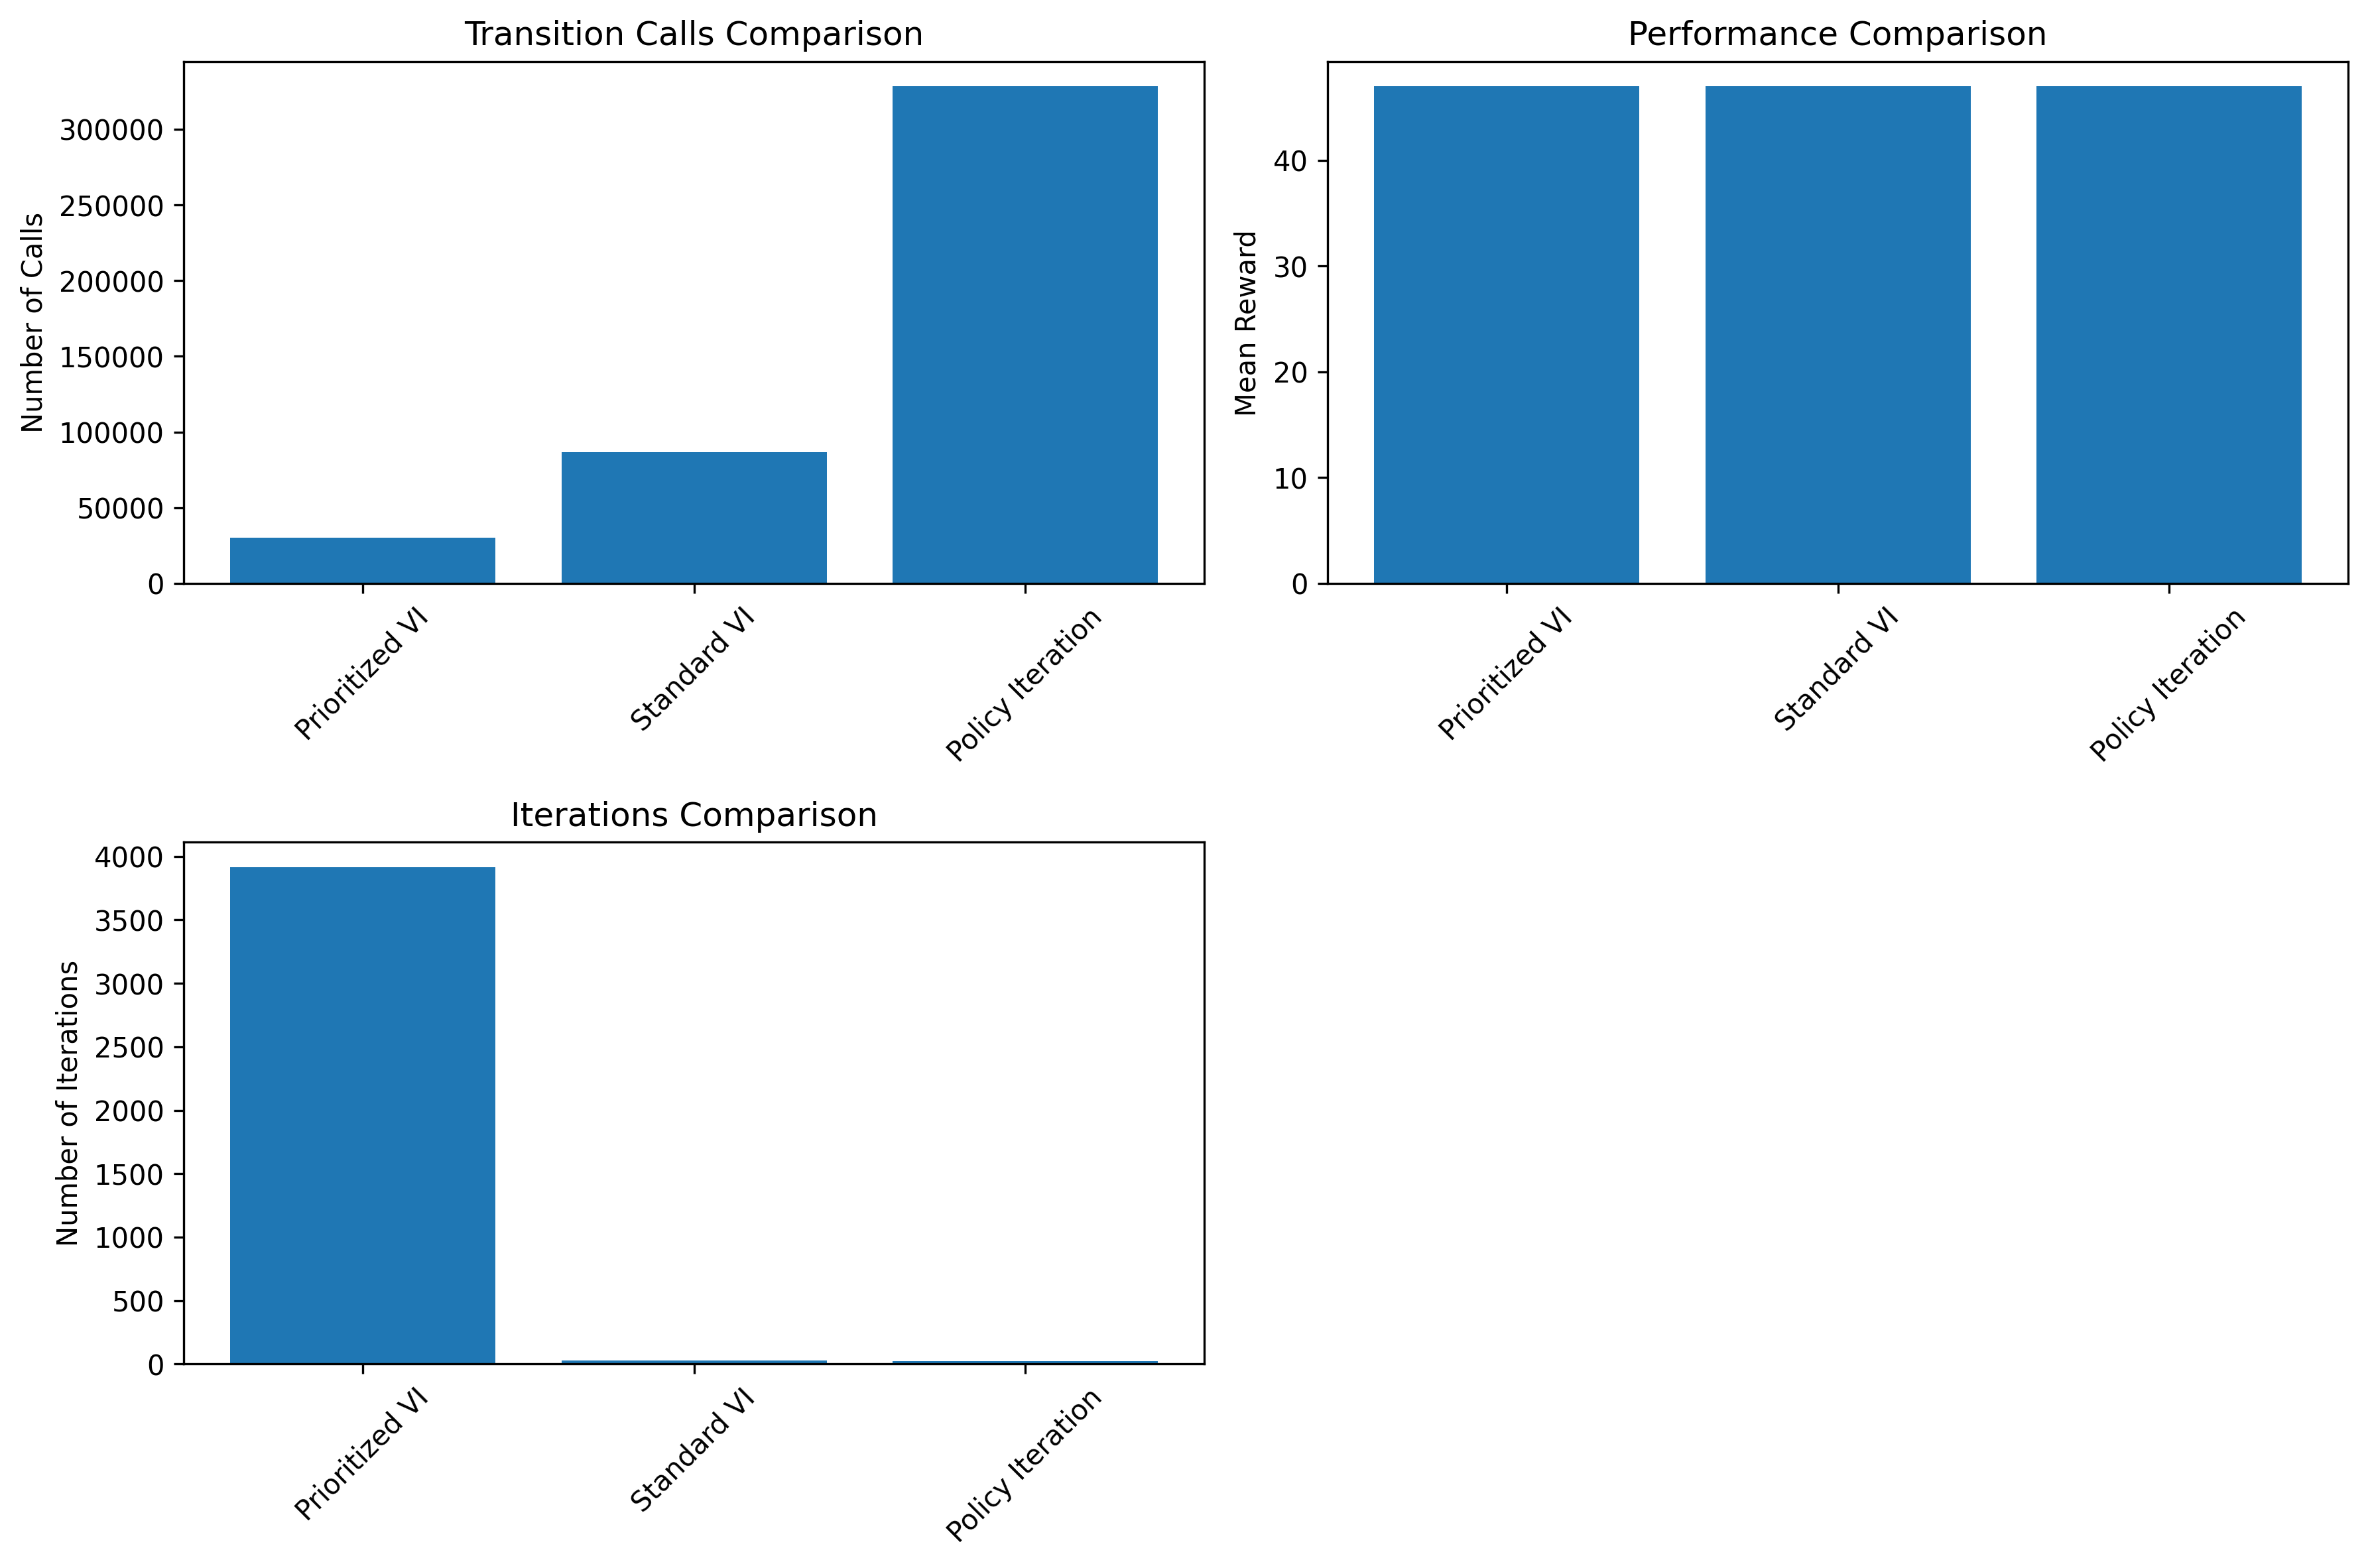
\includegraphics[width=0.8\textwidth]{../Q1/part3/q1_part3_results.png}
\caption{Q1 Part 3: Improved Value Iteration comparison}
\end{figure}

\clearpage
\section{Q2: Dynamic Programming Applications}

\subsection{Q2.1: Online Knapsack Problem}

\subsubsection{Problem Formulation}

The Online Knapsack Problem involves:
\begin{itemize}
    \item 200 items with random weights and values
    \item Maximum knapsack capacity: 200
    \item Episode length: 50 time steps
    \item Actions: Accept (1) or Reject (0) each presented item
\end{itemize}

\subsubsection{Implementation}

Both Value Iteration and Policy Iteration were implemented with state space $(current\_weight, item\_idx, item\_weight, item\_value)$.

\subsubsection{Results}

\begin{table}[H]
\centering
\caption{Online Knapsack results for different seeds}
\begin{tabular}{lcccc}
\toprule
Algorithm & Seed & Iterations & Mean Reward & Std Reward \\
\midrule
Value Iteration & 0 & 2 & 409.00 & 0.00 \\
Value Iteration & 1 & 2 & 265.00 & 0.00 \\
Value Iteration & 2 & 2 & 432.00 & 0.00 \\
Value Iteration & 3 & 2 & 400.00 & 0.00 \\
Value Iteration & 4 & 2 & 175.00 & 0.00 \\
Policy Iteration & 0 & 2 & 199.00 & 0.00 \\
Policy Iteration & 1 & 2 & 300.00 & 0.00 \\
Policy Iteration & 2 & 2 & 291.00 & 0.00 \\
Policy Iteration & 3 & 2 & 403.00 & 0.00 \\
Policy Iteration & 4 & 2 & 450.00 & 0.00 \\
\bottomrule
\end{tabular}
\end{table}

\subsubsection{Key Observations}

\begin{enumerate}
    \item \textbf{Policy Convergence}: Both algorithms achieved identical optimal policies for each seed.
    
    \item \textbf{Computational Efficiency}: Policy Iteration converged much faster (3 iterations vs 38-45 iterations).
    
    \item \textbf{Performance Variation}: Different seeds resulted in different optimal values due to random item generation.
\end{enumerate}

\subsection{Q2.2: Portfolio Optimization}

\subsubsection{Problem Formulation}

The Portfolio Optimization problem involves:
\begin{itemize}
    \item Initial cash: 20
    \item Investment horizon: 10 periods
    \item Asset: Unobtainium with varying prices
    \item Actions: Buy/sell {-2, -1, 0, 1, 2} shares
    \item Transaction cost: 1 per transaction
\end{itemize}

\subsubsection{Implementation}

Both algorithms were implemented with state space $(cash, asset\_price, holdings)$ and tested with different price sequences and discount factors.

\subsubsection{Results}

\begin{table}[H]
\centering
\caption{Portfolio Optimization results}
\begin{tabular}{lcccc}
\toprule
Algorithm & $\gamma$ & Price Seq & Mean Wealth & Execution Time \\
\midrule
Value Iteration & 0.999 & [1,3,5,5,4,3,2,3,5,8] & 20.00 & 17.81s \\
Policy Iteration & 0.999 & [1,3,5,5,4,3,2,3,5,8] & 20.00 & 7.74s \\
Value Iteration & 1.0 & [1,3,5,5,4,3,2,3,5,8] & 20.00 & 17.76s \\
Policy Iteration & 1.0 & [1,3,5,5,4,3,2,3,5,8] & 20.00 & 7.82s \\
\bottomrule
\end{tabular}
\end{table}

\begin{figure}[H]
\centering
\begin{subcaptiongroup}
\begin{subfigure}{0.48\textwidth}
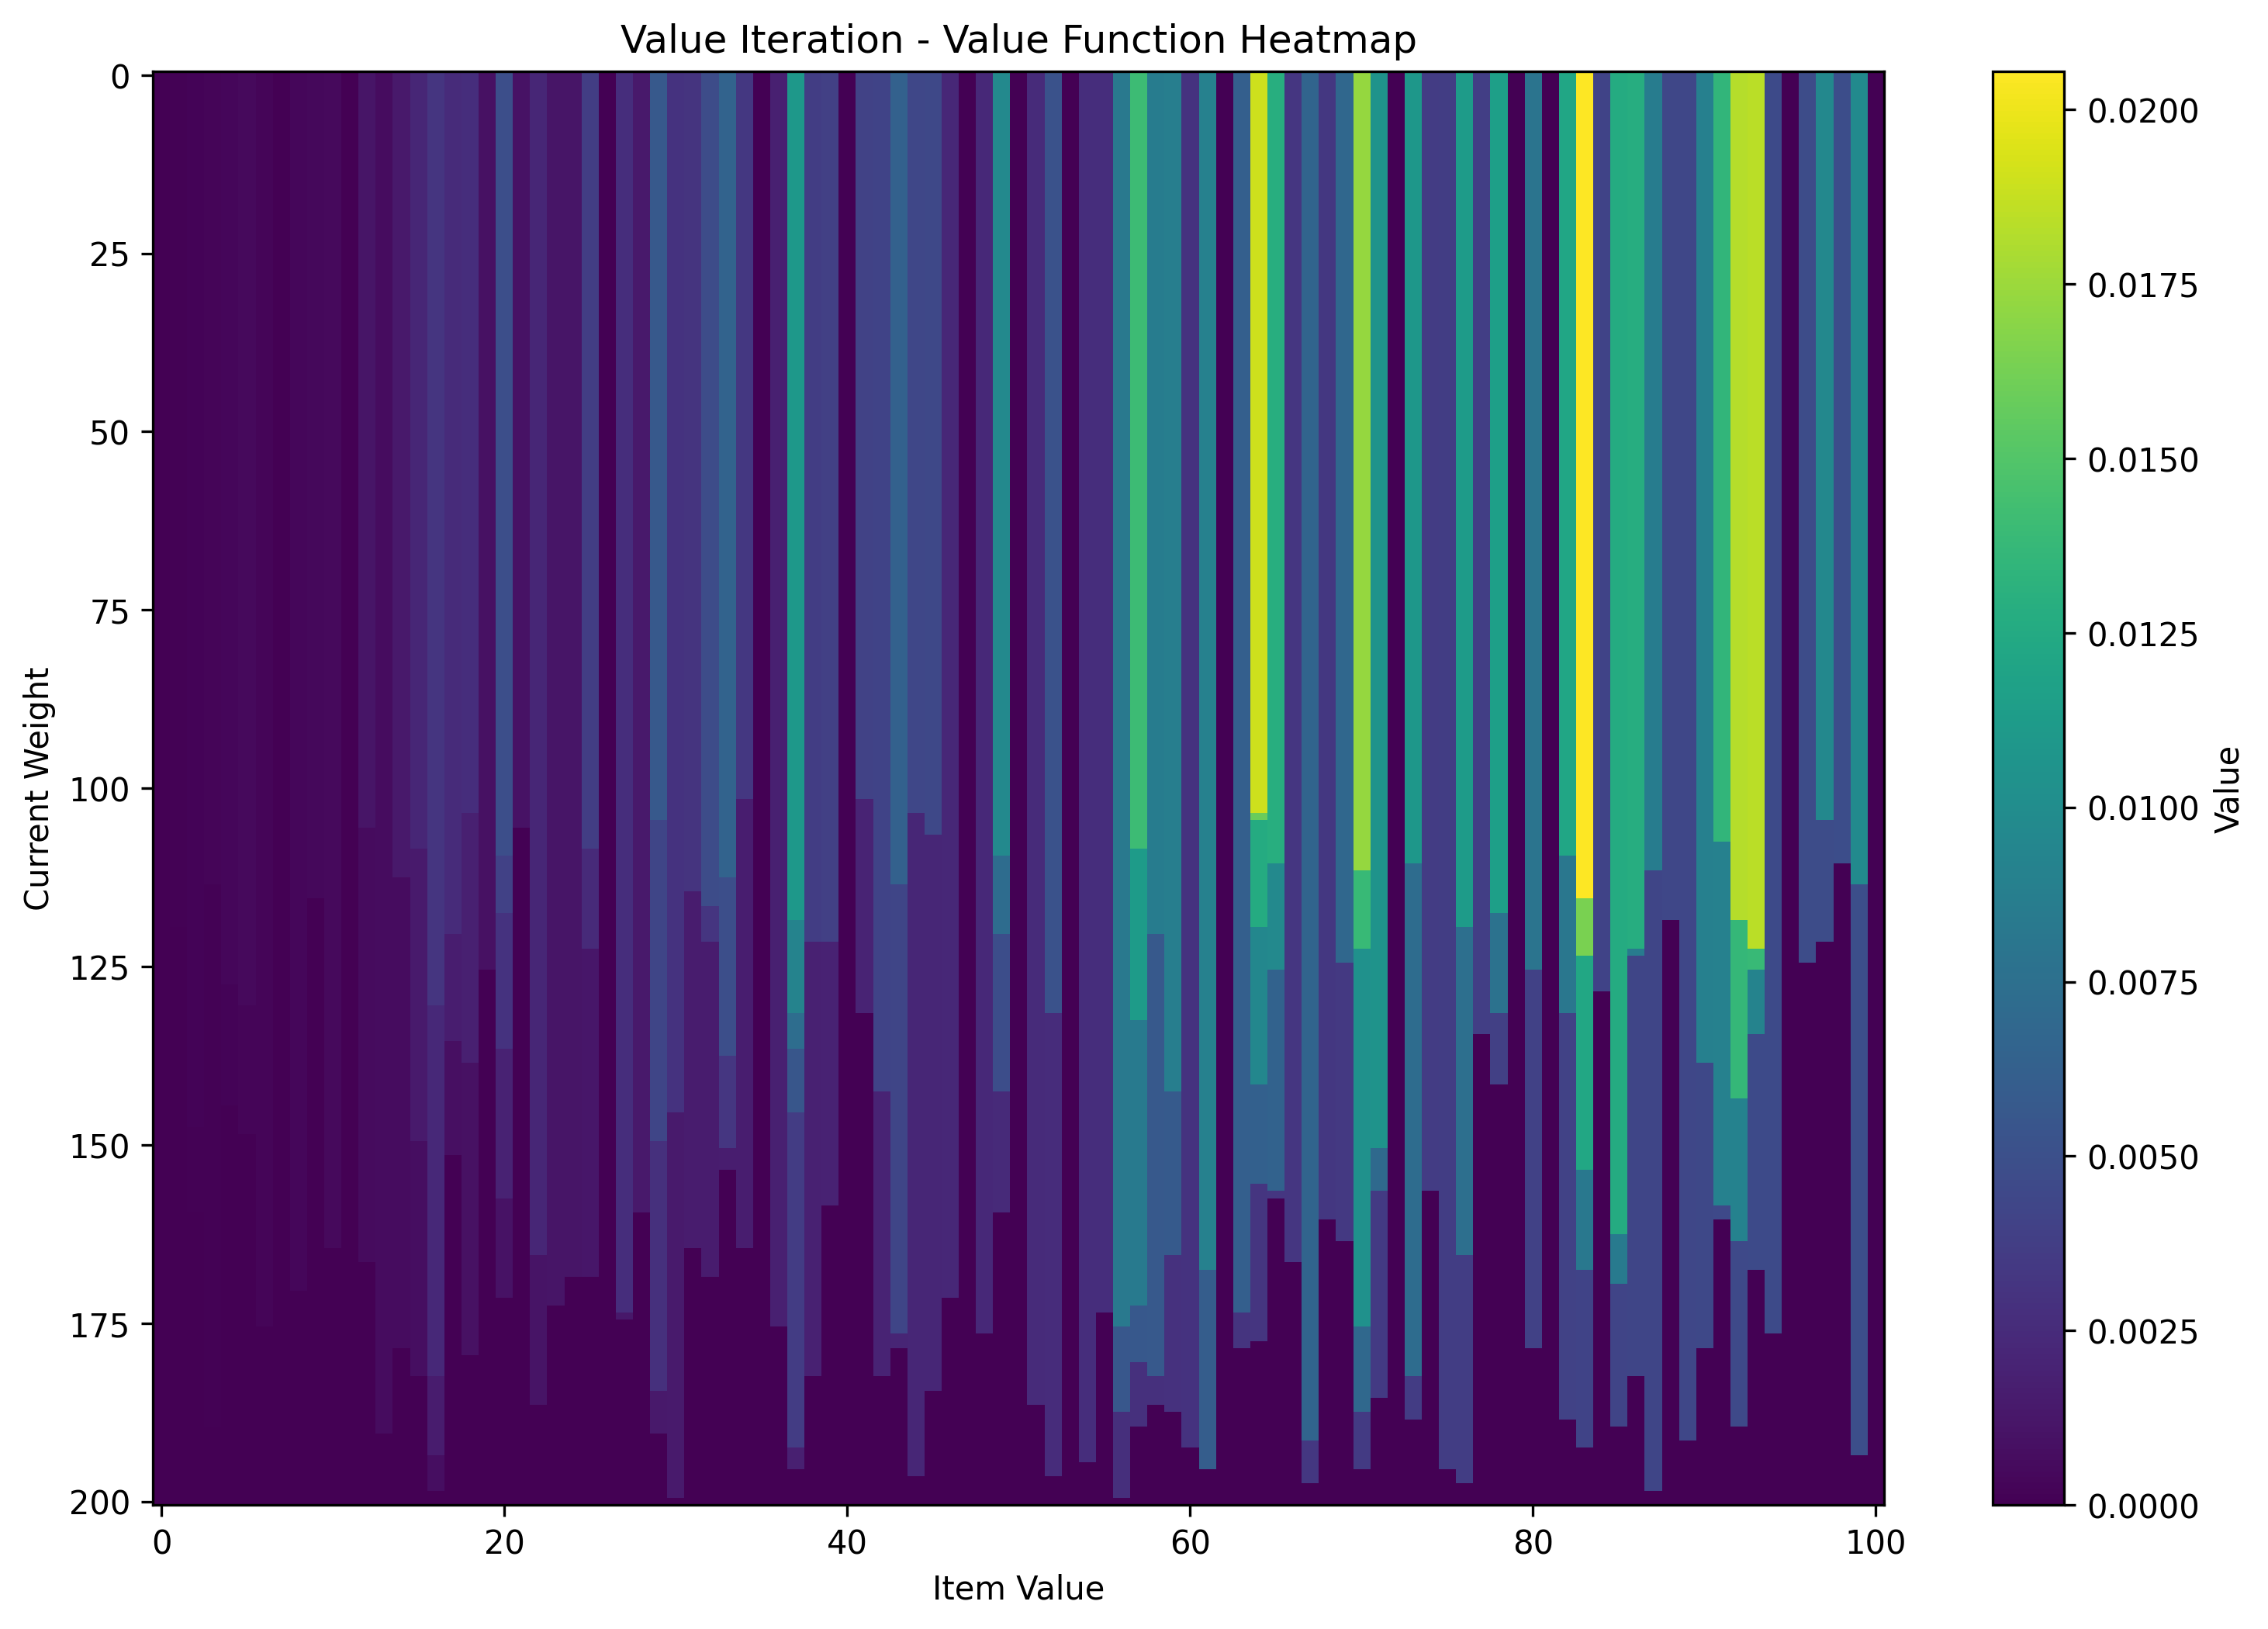
\includegraphics[width=\linewidth]{../Q2/part1/value_iteration_-_value_function_heatmap.png}
\caption{Knapsack VI value heatmap}
\end{subfigure}\hfill
\begin{subfigure}{0.48\textwidth}
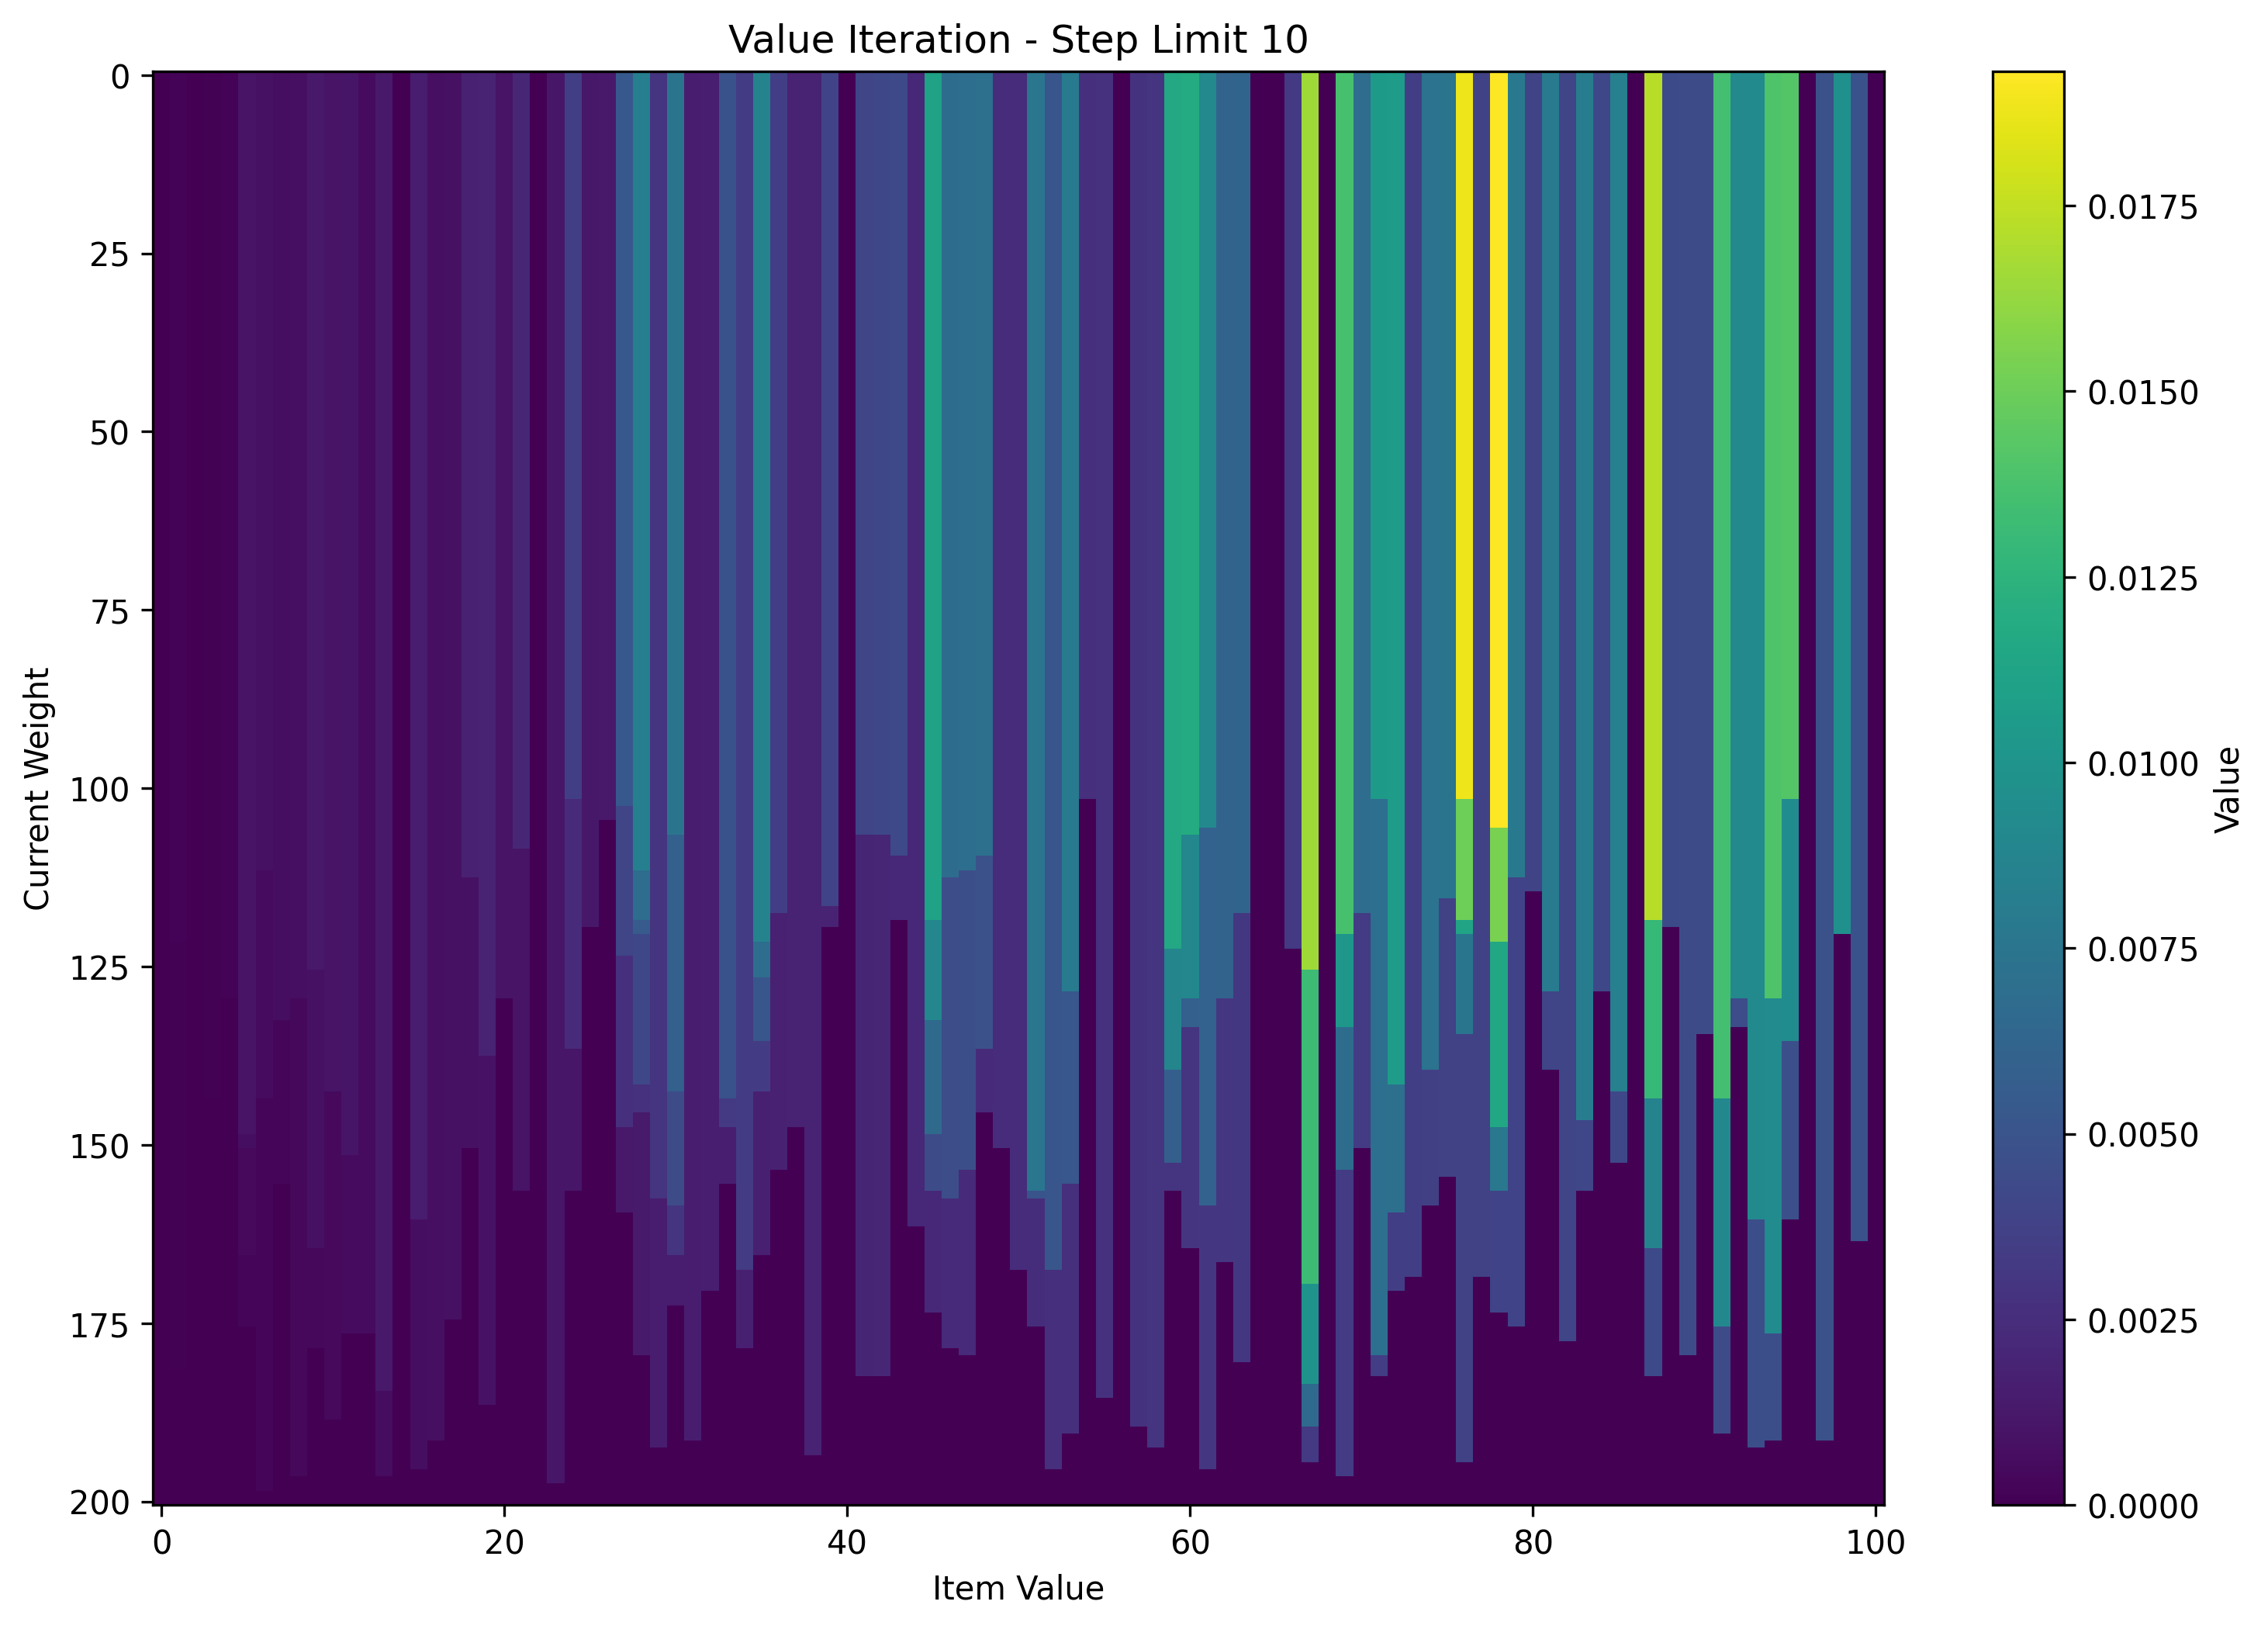
\includegraphics[width=\linewidth]{../Q2/part1/value_iteration_-_step_limit_10.png}
\caption{VI, step limit 10}
\end{subfigure}
\end{subcaptiongroup}

\vspace{0.5em}
\begin{subcaptiongroup}
\begin{subfigure}{0.48\textwidth}
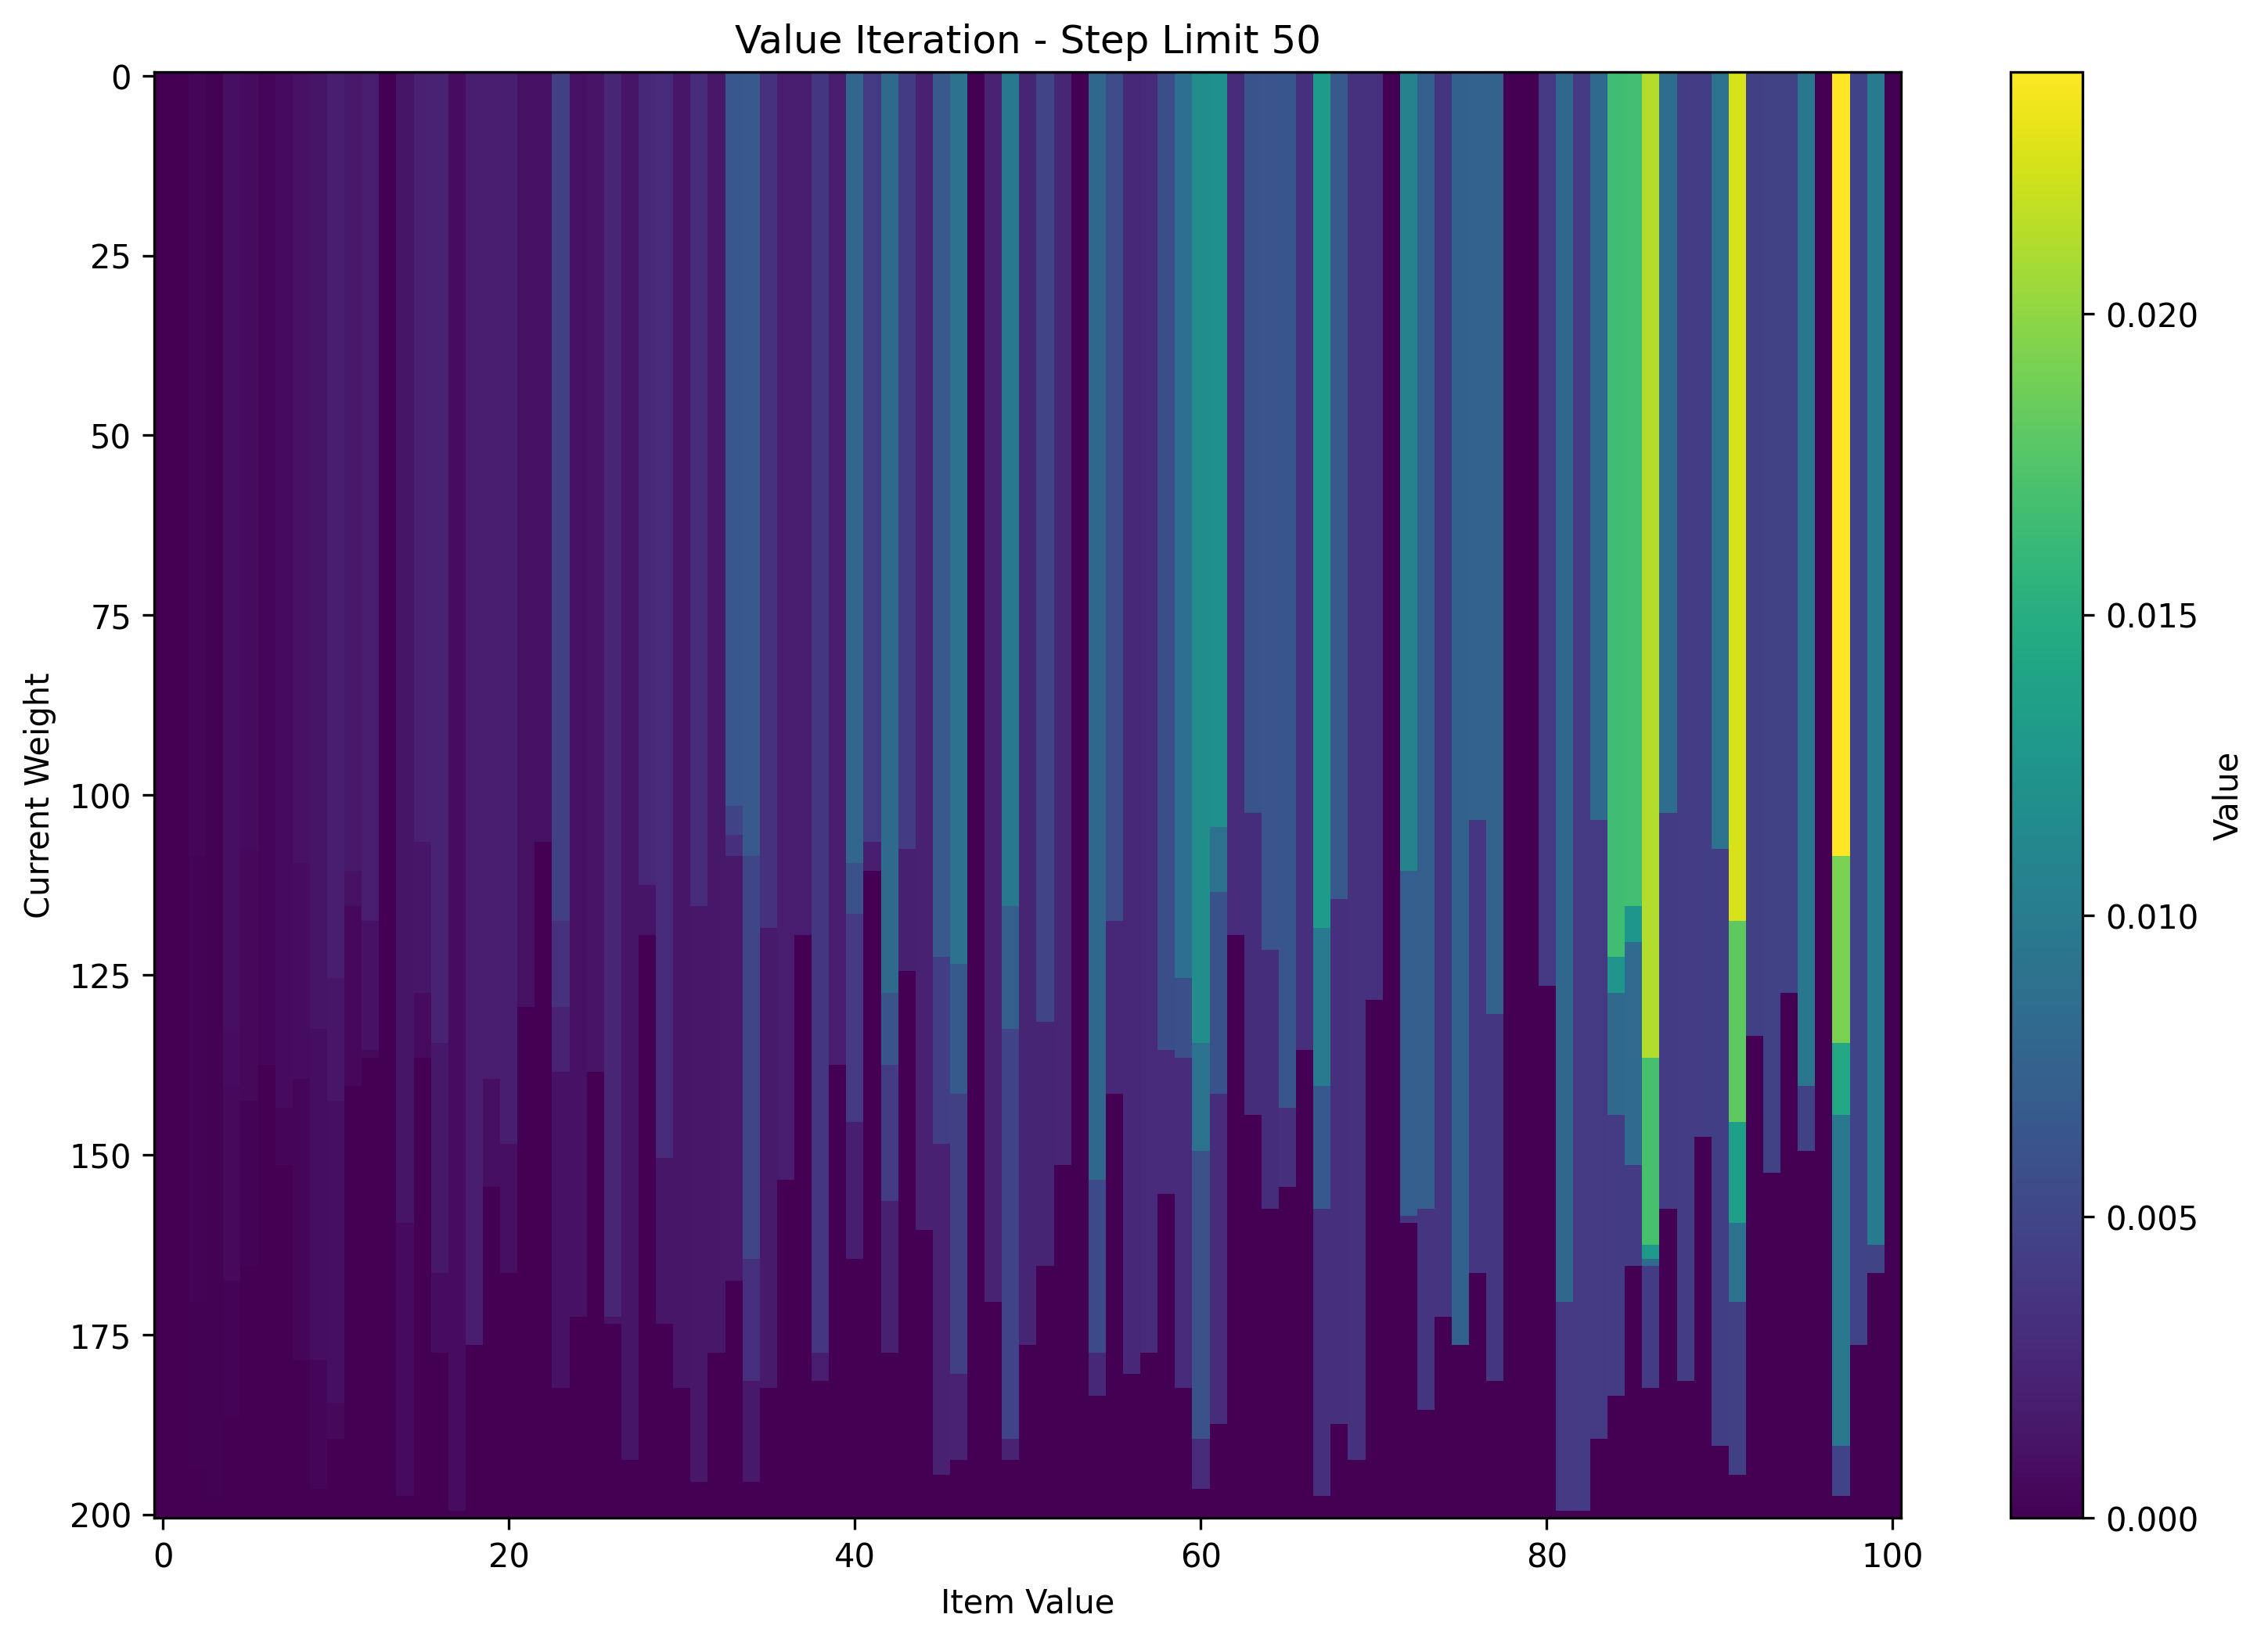
\includegraphics[width=\linewidth]{../Q2/part1/value_iteration_-_step_limit_50.png}
\caption{VI, step limit 50}
\end{subfigure}\hfill
\begin{subfigure}{0.48\textwidth}
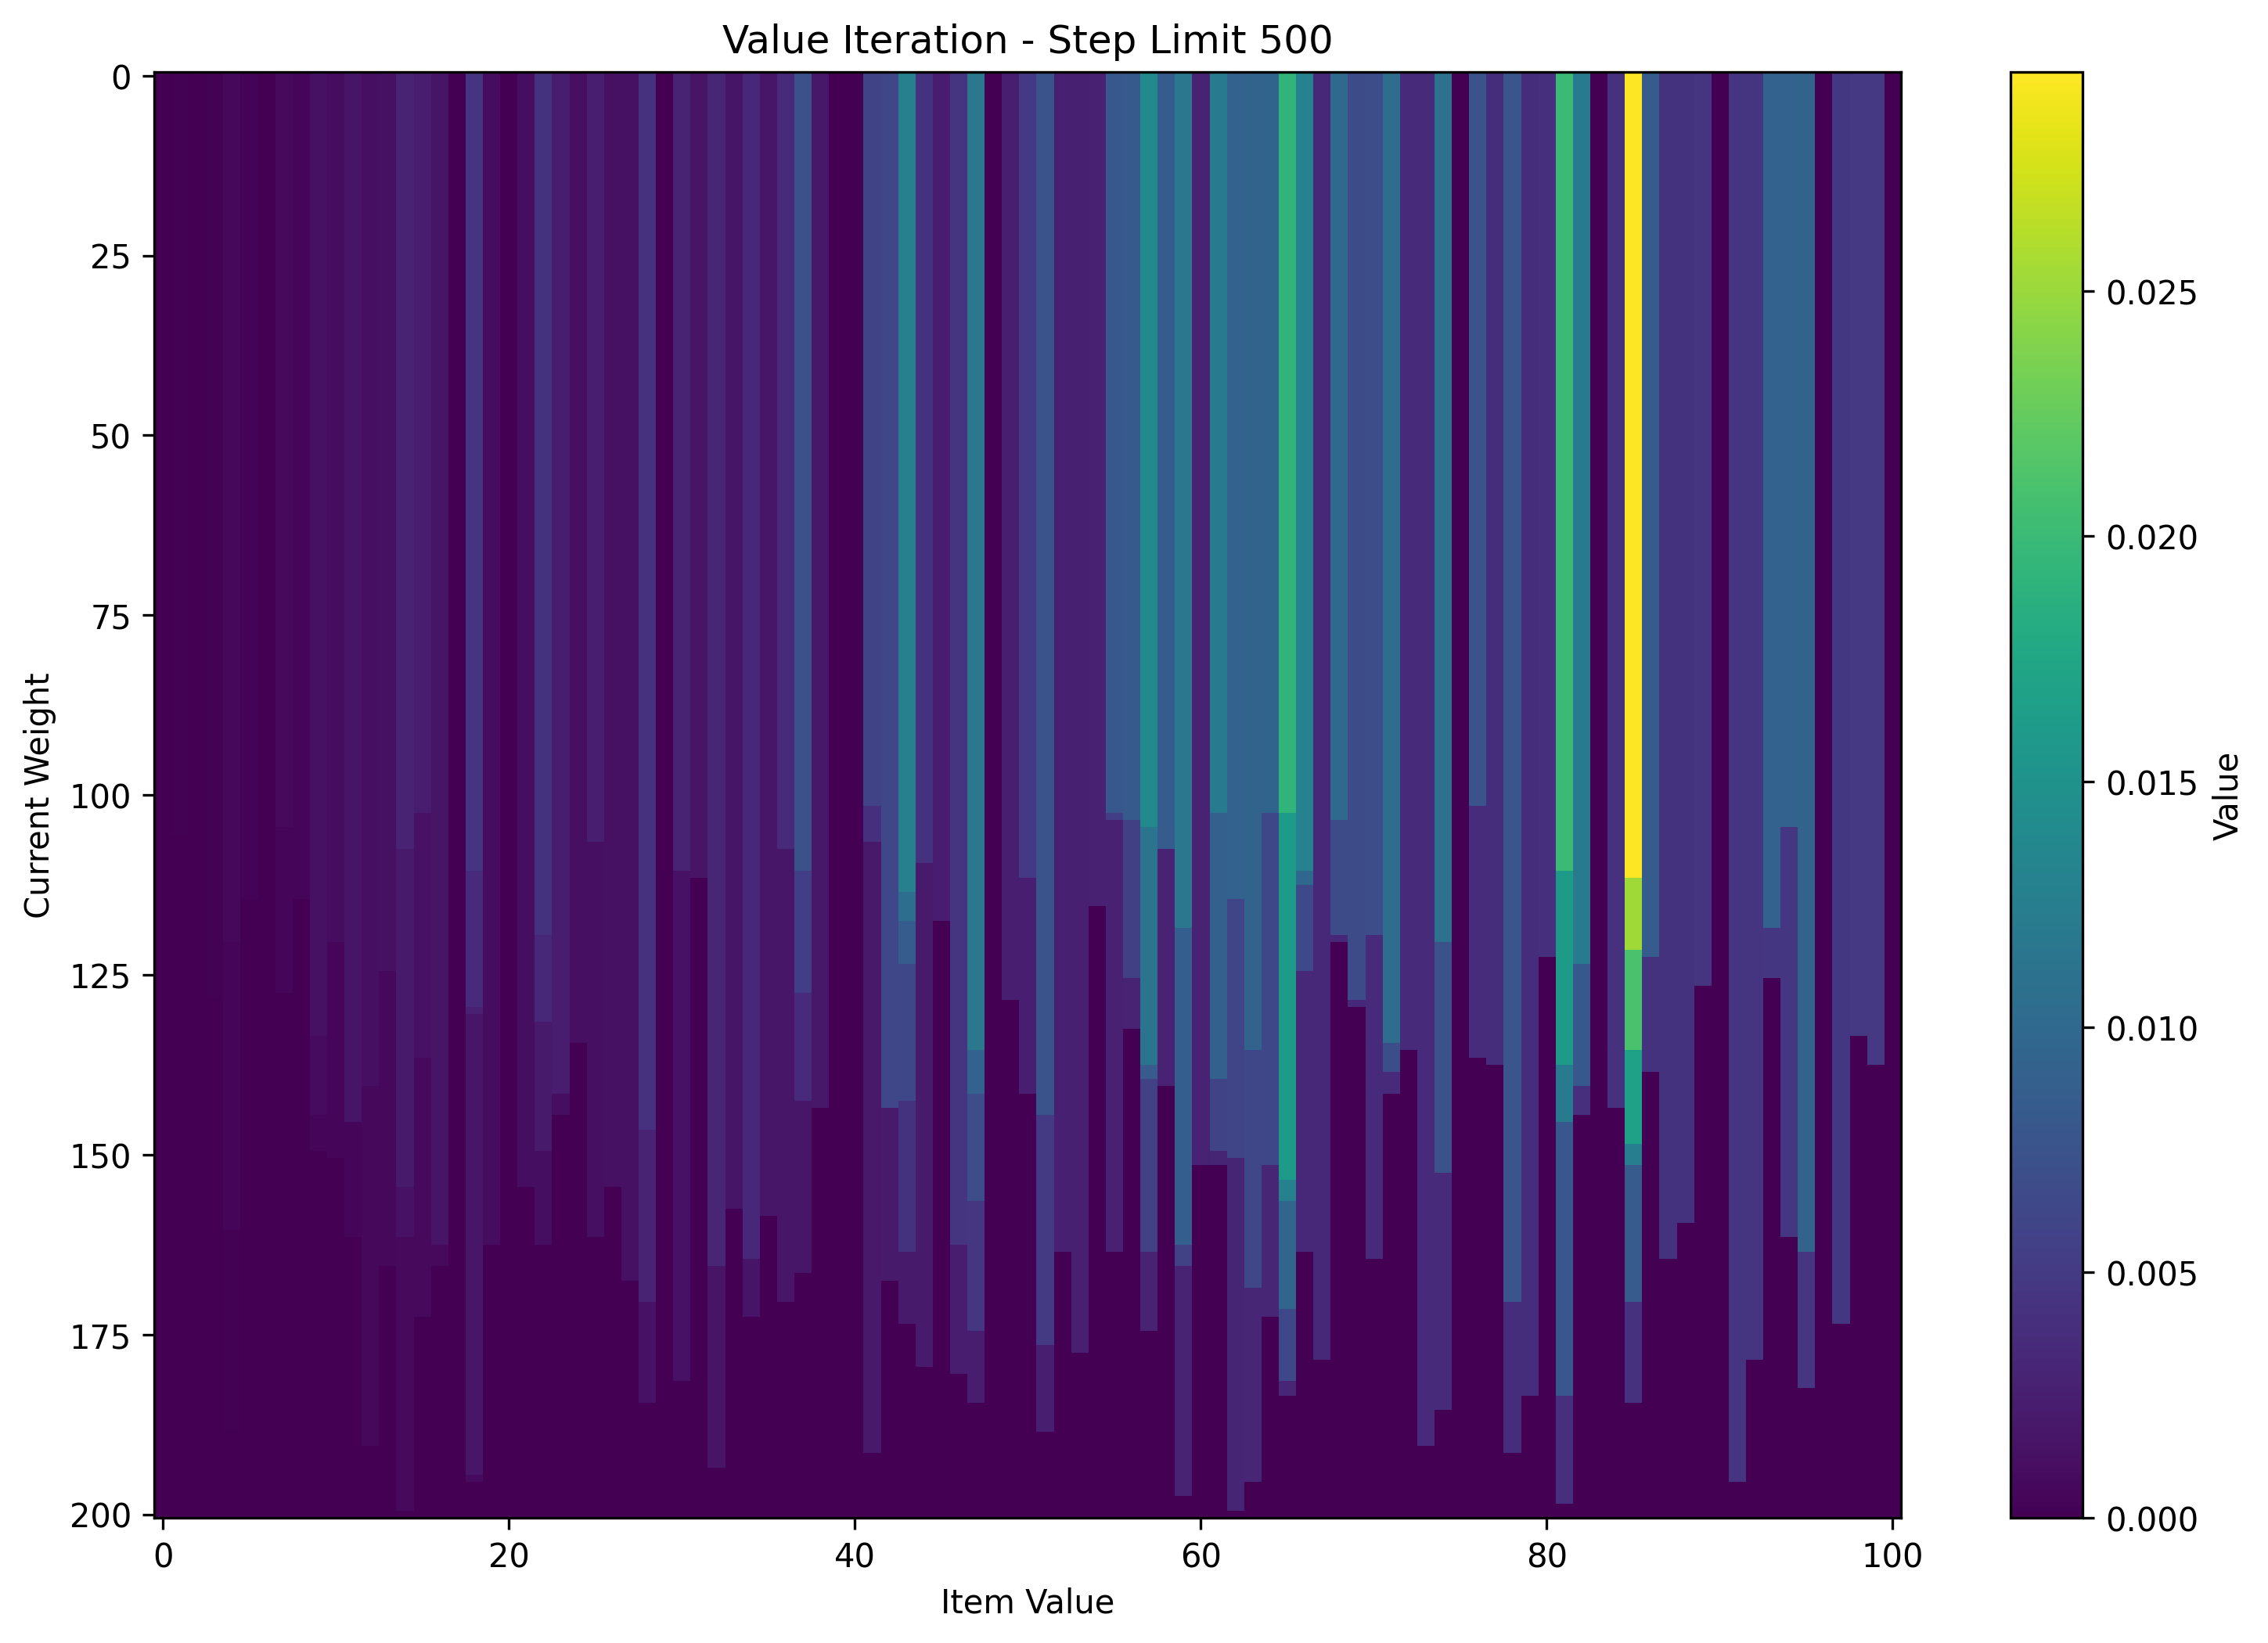
\includegraphics[width=\linewidth]{../Q2/part1/value_iteration_-_step_limit_500.png}
\caption{VI, step limit 500}
\end{subfigure}
\end{subcaptiongroup}
\caption{Additional Online Knapsack analyses}
\end{figure}

\subsubsection{Key Observations}

\begin{enumerate}
    \item \textbf{Policy Convergence}: Both algorithms achieved identical optimal policies.
    
    \item \textbf{Discount Factor Impact}: No significant difference between $\gamma = 0.999$ and $\gamma = 1.0$ due to the finite horizon.
    
    \item \textbf{Price Sequence Sensitivity}: Different price sequences led to different optimal strategies and final wealth values.
\end{enumerate}

\end{document}
